\chapter{Codebase Health Assessment --- 2026-04-05}\label{record-411}

\noindent{\footnotesize\color{BookMuted}\path{docs/audits/2026-04-05-codebase-health-assessment.md}\par}\smallskip

\emph{Two-phase assessment of bijou's external DX and internal structural health, conducted after shipping RE-007 and the perf-gradient stress test.}

\section{0. Executive Report Card}\label{record-411-executive-report-card}

\begin{center}
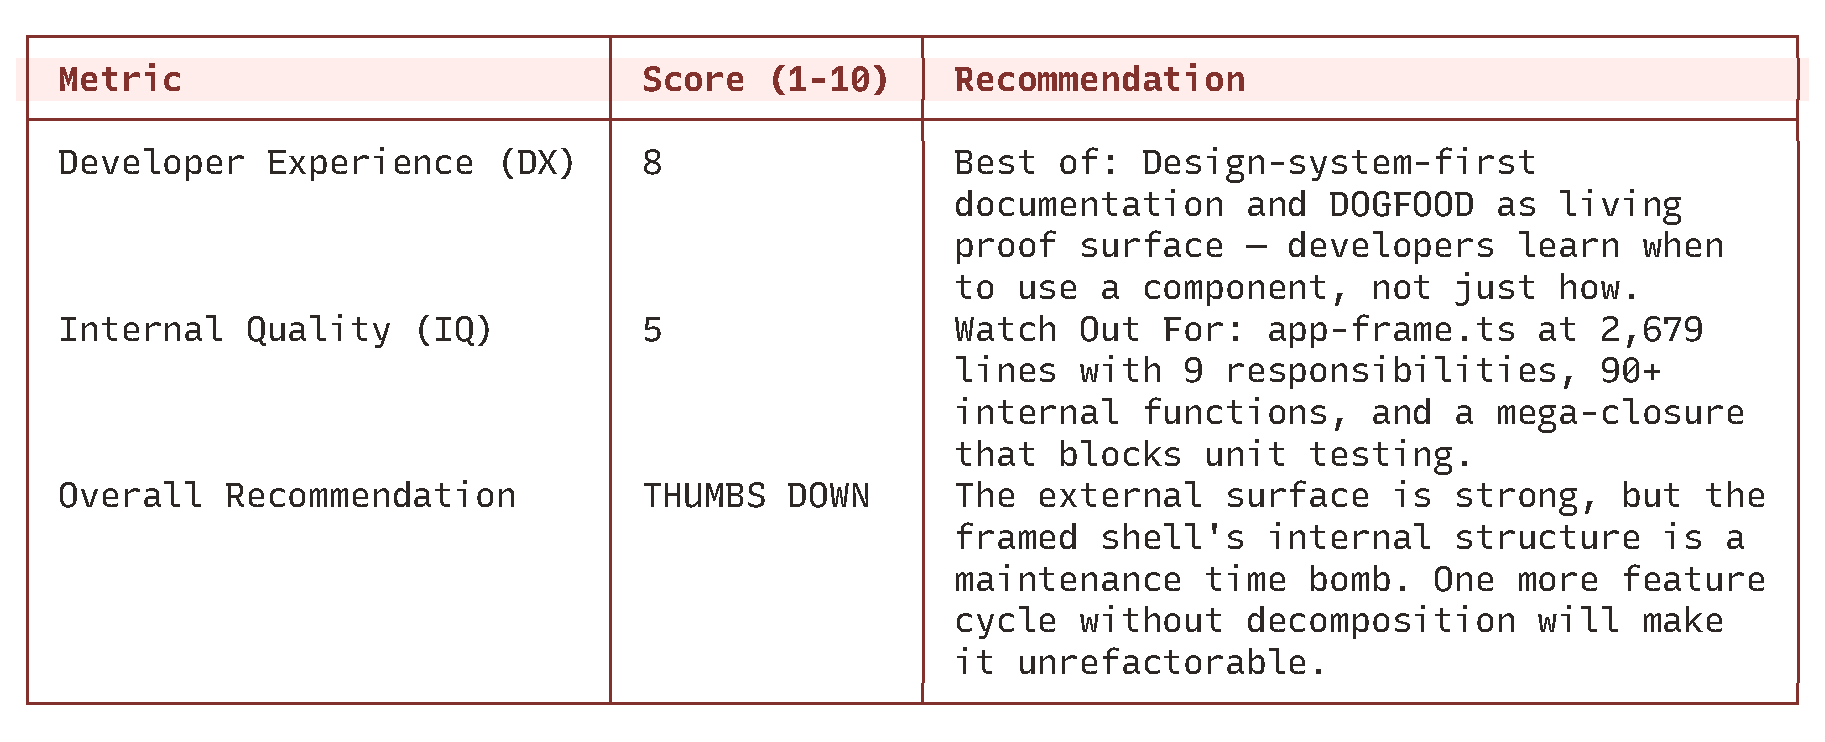
\includegraphics[width=\linewidth]{figures/tables/table-081-g1-1.pdf}
\par\smallskip{\scriptsize\color{BookMuted}Rows 1–3. Actual Bijou table component.}
\end{center}


\begin{center}\rule{0.5\linewidth}{0.5pt}\end{center}

\section{1. DX: Ergonomics \& Interface Clarity}\label{record-411-dx-ergonomics-interface-clarity}

\subsection{1.1. Time-to-Value --- 7/10}\label{record-411-time-to-value-710}

A working TUI app requires three pieces: \texttt{i\allowbreak{}n\allowbreak{}i\allowbreak{}t\allowbreak{}D\allowbreak{}e\allowbreak{}f\allowbreak{}a\allowbreak{}u\allowbreak{}l\allowbreak{}t\allowbreak{}C\allowbreak{}o\allowbreak{}n\allowbreak{}t\allowbreak{}e\allowbreak{}x\allowbreak{}t\allowbreak{}(\allowbreak{})}, an \texttt{A\allowbreak{}p\allowbreak{}p\allowbreak{}<\allowbreak{}M\allowbreak{}o\allowbreak{}d\allowbreak{}e\allowbreak{}l\allowbreak{},\allowbreak{} \allowbreak{}M\allowbreak{}s\allowbreak{}g\allowbreak{}>} object, and \texttt{r\allowbreak{}u\allowbreak{}n\allowbreak{}(\allowbreak{}a\allowbreak{}p\allowbreak{}p\allowbreak{})}. The counter example is 42 lines. Good.

The problem is \texttt{i\allowbreak{}n\allowbreak{}i\allowbreak{}t\allowbreak{}D\allowbreak{}e\allowbreak{}f\allowbreak{}a\allowbreak{}u\allowbreak{}l\allowbreak{}t\allowbreak{}C\allowbreak{}o\allowbreak{}n\allowbreak{}t\allowbreak{}e\allowbreak{}x\allowbreak{}t\allowbreak{}(\allowbreak{})}. It's a mandatory side-effecting call that every app must remember. If you forget it, you get a cryptic error about missing context. This should be automatic or fail with a clear message and a fix instruction.

The scaffolding path (\texttt{n\allowbreak{}p\allowbreak{}m\allowbreak{} \allowbreak{}c\allowbreak{}r\allowbreak{}e\allowbreak{}a\allowbreak{}t\allowbreak{}e\allowbreak{} \allowbreak{}b\allowbreak{}i\allowbreak{}j\allowbreak{}o\allowbreak{}u\allowbreak{}-\allowbreak{}t\allowbreak{}u\allowbreak{}i\allowbreak{}-\allowbreak{}a\allowbreak{}p\allowbreak{}p\allowbreak{}@\allowbreak{}l\allowbreak{}a\allowbreak{}t\allowbreak{}e\allowbreak{}s\allowbreak{}t}) handles this implicitly, but anyone integrating bijou into an existing project hits this wall.

\textbf{Backlog:} \href{https://github.com/flyingrobots/bijou/blob/cbd70612140e7a450d764b3c7be1c6af878b99bc/docs/method/graveyard/legacy-backlog/inbox/DX-009-context-auto-init-and-error-messages.md}{DX-009}

\subsection{1.2. Principle of Least Astonishment --- Frame key priority}\label{record-411-principle-of-least-astonishment-frame-key-priority}

\texttt{k\allowbreak{}e\allowbreak{}y\allowbreak{}P\allowbreak{}r\allowbreak{}i\allowbreak{}o\allowbreak{}r\allowbreak{}i\allowbreak{}t\allowbreak{}y} defaults to \texttt{'\allowbreak{}f\allowbreak{}r\allowbreak{}a\allowbreak{}m\allowbreak{}e\allowbreak{}-\allowbreak{}f\allowbreak{}i\allowbreak{}r\allowbreak{}s\allowbreak{}t\allowbreak{}'}, meaning the shell's keybindings (help \texttt{?}, settings \texttt{c\allowbreak{}t\allowbreak{}r\allowbreak{}l\allowbreak{}+\allowbreak{},}, quit \texttt{e\allowbreak{}s\allowbreak{}c\allowbreak{}a\allowbreak{}p\allowbreak{}e}) silently win over the app's page keybindings. A developer who binds \texttt{?} to ``show info'' in their page will never see it fire. The default is sensible for shell apps but surprising for developers who expect their app's keys to be primary.

There is no warning when a page binding collides with a frame binding. The key is silently consumed by the frame.

\textbf{Backlog:} \href{https://github.com/flyingrobots/bijou/blob/cbd70612140e7a450d764b3c7be1c6af878b99bc/docs/method/graveyard/legacy-backlog/inbox/DX-009-context-auto-init-and-error-messages.md}{DX-009}

\subsection{1.3. Error Usability --- Missing context}\label{record-411-error-usability-missing-context}

When \texttt{g\allowbreak{}e\allowbreak{}t\allowbreak{}D\allowbreak{}e\allowbreak{}f\allowbreak{}a\allowbreak{}u\allowbreak{}l\allowbreak{}t\allowbreak{}C\allowbreak{}o\allowbreak{}n\allowbreak{}t\allowbreak{}e\allowbreak{}x\allowbreak{}t\allowbreak{}(\allowbreak{})} is called before \texttt{i\allowbreak{}n\allowbreak{}i\allowbreak{}t\allowbreak{}D\allowbreak{}e\allowbreak{}f\allowbreak{}a\allowbreak{}u\allowbreak{}l\allowbreak{}t\allowbreak{}C\allowbreak{}o\allowbreak{}n\allowbreak{}t\allowbreak{}e\allowbreak{}x\allowbreak{}t\allowbreak{}(\allowbreak{})}:

\begin{CodeBlock}
Error: No default BijouContext has been set.
\end{CodeBlock}

This tells you what's wrong but not how to fix it. A developer unfamiliar with the port architecture won't know what to do next. The error should say:

\begin{CodeBlock}
No default BijouContext has been set.
Call initDefaultContext() from '@flyingrobots/bijou-node' at the top
of your entry file, or pass an explicit ctx to run().
See: https://github.com/flyingrobots/bijou#quick-start
\end{CodeBlock}

\textbf{Backlog:} \href{https://github.com/flyingrobots/bijou/blob/cbd70612140e7a450d764b3c7be1c6af878b99bc/docs/method/graveyard/legacy-backlog/inbox/DX-009-context-auto-init-and-error-messages.md}{DX-009}

\begin{center}\rule{0.5\linewidth}{0.5pt}\end{center}

\section{2. DX: Documentation \& Extendability}\label{record-411-dx-documentation-extendability}

\subsection{2.1. Documentation Gap --- Render pipeline guide}\label{record-411-documentation-gap-render-pipeline-guide}

The render pipeline (the illustrated sequence below) is a powerful extension point but has zero documentation beyond the type definitions. \texttt{c\allowbreak{}o\allowbreak{}n\allowbreak{}f\allowbreak{}i\allowbreak{}g\allowbreak{}u\allowbreak{}r\allowbreak{}e\allowbreak{}P\allowbreak{}i\allowbreak{}p\allowbreak{}e\allowbreak{}l\allowbreak{}i\allowbreak{}n\allowbreak{}e} appears in \texttt{R\allowbreak{}u\allowbreak{}n\allowbreak{}O\allowbreak{}p\allowbreak{}t\allowbreak{}i\allowbreak{}o\allowbreak{}n\allowbreak{}s} but there is no guide showing how to write a custom middleware, what \texttt{R\allowbreak{}e\allowbreak{}n\allowbreak{}d\allowbreak{}e\allowbreak{}r\allowbreak{}S\allowbreak{}t\allowbreak{}a\allowbreak{}t\allowbreak{}e} fields are available, or how stages interact.

% Presentation of original arrow notation. See flow-manifest.json.
\begin{center}
\begin{tikzpicture}[book flow node/.style={draw=BookHeading,line width=.65pt,fill=BookPanel,rounded corners=1.5pt,align=center,inner sep=5pt,minimum height=10mm,font=\fontsize{9}{11}\selectfont,execute at begin node={\hyphenpenalty=10000\exhyphenpenalty=10000}},book flow edge/.style={-{Latex[length=2mm]},draw=BookHeading,line width=.7pt}]
\node[book flow node,text width=96mm] (n0) at (0,0.0) {Layout};
\node[book flow node,text width=96mm] (n1) at (0,-1.55) {Paint};
\node[book flow node,text width=96mm] (n2) at (0,-3.1) {Post\allowbreak{}Process};
\node[book flow node,text width=96mm] (n3) at (0,-4.65) {Diff};
\node[book flow node,text width=96mm] (n4) at (0,-6.2) {Output};
\draw[book flow edge] (n0) -- (n1);
\draw[book flow edge] (n1) -- (n2);
\draw[book flow edge] (n2) -- (n3);
\draw[book flow edge] (n3) -- (n4);
\end{tikzpicture}
\end{center}


The perf-gradient demo proved this gap --- we could not instrument the pipeline from outside to measure per-stage timing.

Other documentation is excellent: - Design-system-first approach is strong - DOGFOOD as living proof surface - Multiple entry points (quick start, architecture, design system) - \texttt{d\allowbreak{}o\allowbreak{}c\allowbreak{}s\allowbreak{}/\allowbreak{}R\allowbreak{}E\allowbreak{}A\allowbreak{}D\allowbreak{}M\allowbreak{}E\allowbreak{}.\allowbreak{}m\allowbreak{}d} provides explicit audit rules

\textbf{Backlog:} \href{https://github.com/flyingrobots/bijou/blob/cbd70612140e7a450d764b3c7be1c6af878b99bc/docs/method/graveyard/legacy-backlog/inbox/DX-008-render-pipeline-guide.md}{DX-008}

\subsection{2.2. Customization --- 8/10}\label{record-411-customization-810}

\textbf{Strongest:} \texttt{c\allowbreak{}o\allowbreak{}n\allowbreak{}f\allowbreak{}i\allowbreak{}g\allowbreak{}u\allowbreak{}r\allowbreak{}e\allowbreak{}P\allowbreak{}i\allowbreak{}p\allowbreak{}e\allowbreak{}l\allowbreak{}i\allowbreak{}n\allowbreak{}e} + \texttt{R\allowbreak{}e\allowbreak{}n\allowbreak{}d\allowbreak{}e\allowbreak{}r\allowbreak{}M\allowbreak{}i\allowbreak{}d\allowbreak{}d\allowbreak{}l\allowbreak{}e\allowbreak{}w\allowbreak{}a\allowbreak{}r\allowbreak{}e}. Non-invasive, composable, and the grayscale filter is a canonical example. The \texttt{C\allowbreak{}r\allowbreak{}e\allowbreak{}a\allowbreak{}t\allowbreak{}e\allowbreak{}F\allowbreak{}r\allowbreak{}a\allowbreak{}m\allowbreak{}e\allowbreak{}d\allowbreak{}A\allowbreak{}p\allowbreak{}p\allowbreak{}O\allowbreak{}p\allowbreak{}t\allowbreak{}i\allowbreak{}o\allowbreak{}n\allowbreak{}s} is remarkably comprehensive --- headerStyle, observeKey, overlayFactory, settings, notificationCenter all allow deep customization without forking.

\textbf{Weakest:} Sub-app composition via \texttt{m\allowbreak{}o\allowbreak{}u\allowbreak{}n\allowbreak{}t\allowbreak{}(\allowbreak{})} / \texttt{m\allowbreak{}a\allowbreak{}p\allowbreak{}C\allowbreak{}m\allowbreak{}d\allowbreak{}s\allowbreak{}(\allowbreak{})}. It works but requires manual message wiring that's easy to get wrong. There is no type-level guarantee that all sub-app messages are mapped, and forgotten mappings cause silent message drops.

\textbf{Backlog:} \href{https://github.com/flyingrobots/bijou/blob/cbd70612140e7a450d764b3c7be1c6af878b99bc/docs/method/graveyard/legacy-backlog/cool-ideas/DX-010-typed-subapp-adapter.md}{DX-010}

\begin{center}\rule{0.5\linewidth}{0.5pt}\end{center}

\section{3. Internal Quality: Architecture \& Maintainability}\label{record-411-internal-quality-architecture-maintainability}

\subsection{3.1. Technical Debt Hotspot --- app-frame.ts (2,679 lines)}\label{record-411-technical-debt-hotspot-app-frame.ts-2679-lines}

This is the single biggest structural problem in the codebase. The file has grown through six runtime-engine cycles (RE-001 to RE-007) as each slice added routing, layout, and buffer infrastructure into the same closure. It now has:

\begin{itemize}
\tightlist
\item
  9 responsibilities (routing, rendering, state, command dispatch, settings, notifications, help, overlays, transitions)
\item
  90+ internal functions inside a single \texttt{c\allowbreak{}r\allowbreak{}e\allowbreak{}a\allowbreak{}t\allowbreak{}e\allowbreak{}F\allowbreak{}r\allowbreak{}a\allowbreak{}m\allowbreak{}e\allowbreak{}d\allowbreak{}A\allowbreak{}p\allowbreak{}p\allowbreak{}(\allowbreak{})} closure
\item
  38 import statements
\item
  A circular import with \texttt{a\allowbreak{}p\allowbreak{}p\allowbreak{}-\allowbreak{}f\allowbreak{}r\allowbreak{}a\allowbreak{}m\allowbreak{}e\allowbreak{}-\allowbreak{}t\allowbreak{}y\allowbreak{}p\allowbreak{}e\allowbreak{}s\allowbreak{}.\allowbreak{}t\allowbreak{}s}
\item
  No individual function can be unit-tested
\end{itemize}

\textbf{Backlog:} \href{https://github.com/flyingrobots/bijou/blob/cbd70612140e7a450d764b3c7be1c6af878b99bc/docs/method/graveyard/legacy-backlog/bad-code/DX-007-decompose-app-frame-mega-closure.md}{DX-007}

\subsection{3.2. Abstraction Violation --- Circular import}\label{record-411-abstraction-violation-circular-import}

\texttt{a\allowbreak{}p\allowbreak{}p\allowbreak{}-\allowbreak{}f\allowbreak{}r\allowbreak{}a\allowbreak{}m\allowbreak{}e\allowbreak{}-\allowbreak{}t\allowbreak{}y\allowbreak{}p\allowbreak{}e\allowbreak{}s\allowbreak{}.\allowbreak{}t\allowbreak{}s} imports \texttt{F\allowbreak{}r\allowbreak{}a\allowbreak{}m\allowbreak{}e\allowbreak{}M\allowbreak{}o\allowbreak{}d\allowbreak{}e\allowbreak{}l} from \texttt{a\allowbreak{}p\allowbreak{}p\allowbreak{}-\allowbreak{}f\allowbreak{}r\allowbreak{}a\allowbreak{}m\allowbreak{}e\allowbreak{}.\allowbreak{}t\allowbreak{}s}, and \texttt{a\allowbreak{}p\allowbreak{}p\allowbreak{}-\allowbreak{}f\allowbreak{}r\allowbreak{}a\allowbreak{}m\allowbreak{}e\allowbreak{}.\allowbreak{}t\allowbreak{}s} imports types from \texttt{a\allowbreak{}p\allowbreak{}p\allowbreak{}-\allowbreak{}f\allowbreak{}r\allowbreak{}a\allowbreak{}m\allowbreak{}e\allowbreak{}-\allowbreak{}t\allowbreak{}y\allowbreak{}p\allowbreak{}e\allowbreak{}s\allowbreak{}.\allowbreak{}t\allowbreak{}s}. TypeScript resolves this for type-only imports, but it couples the type layer to the implementation file and makes refactoring dangerous.

\textbf{Backlog:} \href{https://github.com/flyingrobots/bijou/blob/cbd70612140e7a450d764b3c7be1c6af878b99bc/docs/method/graveyard/legacy-backlog/bad-code/DX-007-decompose-app-frame-mega-closure.md}{DX-007} (addressed as part of the decomposition)

\subsection{3.3. Testability Barrier --- The mega-closure}\label{record-411-testability-barrier-the-mega-closure}

\texttt{c\allowbreak{}r\allowbreak{}e\allowbreak{}a\allowbreak{}t\allowbreak{}e\allowbreak{}F\allowbreak{}r\allowbreak{}a\allowbreak{}m\allowbreak{}e\allowbreak{}d\allowbreak{}A\allowbreak{}p\allowbreak{}p\allowbreak{}(\allowbreak{})} is a 2,000-line closure. Every internal function captures \texttt{o\allowbreak{}p\allowbreak{}t\allowbreak{}i\allowbreak{}o\allowbreak{}n\allowbreak{}s}, \texttt{p\allowbreak{}a\allowbreak{}g\allowbreak{}e\allowbreak{}s\allowbreak{}B\allowbreak{}y\allowbreak{}I\allowbreak{}d}, \texttt{f\allowbreak{}r\allowbreak{}a\allowbreak{}m\allowbreak{}e\allowbreak{}K\allowbreak{}e\allowbreak{}y\allowbreak{}s}, and \texttt{p\allowbreak{}a\allowbreak{}l\allowbreak{}e\allowbreak{}t\allowbreak{}t\allowbreak{}e\allowbreak{}K\allowbreak{}e\allowbreak{}y\allowbreak{}s} via closure. None can be imported, called, or tested independently. The only way to test them is through the full \texttt{a\allowbreak{}p\allowbreak{}p\allowbreak{}.\allowbreak{}i\allowbreak{}n\allowbreak{}i\allowbreak{}t\allowbreak{}(\allowbreak{})} / \texttt{a\allowbreak{}p\allowbreak{}p\allowbreak{}.\allowbreak{}u\allowbreak{}p\allowbreak{}d\allowbreak{}a\allowbreak{}t\allowbreak{}e\allowbreak{}(\allowbreak{})} integration path.

This makes tests: - \textbf{Slow} --- full app initialization for every test case - \textbf{Coarse} --- can't test a single handler without triggering the entire update cycle - \textbf{Fragile} --- a bug in settings focus logic requires debugging through the routing + command buffer + handler table chain

\textbf{Backlog:} \href{https://github.com/flyingrobots/bijou/blob/cbd70612140e7a450d764b3c7be1c6af878b99bc/docs/method/graveyard/legacy-backlog/bad-code/DX-007-decompose-app-frame-mega-closure.md}{DX-007}

\begin{center}\rule{0.5\linewidth}{0.5pt}\end{center}

\section{4. Internal Quality: Risk \& Efficiency}\label{record-411-internal-quality-risk-efficiency}

\subsection{4.1. Critical Flaw --- Mutable surface caches}\label{record-411-critical-flaw-mutable-surface-caches}

Two module-level mutable variables cache \texttt{S\allowbreak{}u\allowbreak{}r\allowbreak{}f\allowbreak{}a\allowbreak{}c\allowbreak{}e} objects:

\begin{CodeBlock}
// app-frame.ts:675
let composedFrameScratch: Surface | null = null;

// app-frame-actions.ts:54
let focusedPaneMeasureScratch: Surface | null = null;
\end{CodeBlock}

If any code path mutates the returned surface after the cache check, the mutation corrupts the cache for subsequent frames. This is a latent state-corruption bug that would manifest as visual glitches with no obvious cause.

The caches are also module-scoped, not instance-scoped. If two \texttt{c\allowbreak{}r\allowbreak{}e\allowbreak{}a\allowbreak{}t\allowbreak{}e\allowbreak{}F\allowbreak{}r\allowbreak{}a\allowbreak{}m\allowbreak{}e\allowbreak{}d\allowbreak{}A\allowbreak{}p\allowbreak{}p} instances existed (unlikely but possible), they would share the same mutable cache.

\textbf{Backlog:} \href{https://github.com/flyingrobots/bijou/blob/cbd70612140e7a450d764b3c7be1c6af878b99bc/docs/method/graveyard/legacy-backlog/bad-code/RE-010-mutable-surface-caches.md}{RE-010}

\subsection{4.2. Efficiency Sink --- renderDiff string concatenation}\label{record-411-efficiency-sink-renderdiff-string-concatenation}

\texttt{r\allowbreak{}e\allowbreak{}n\allowbreak{}d\allowbreak{}e\allowbreak{}r\allowbreak{}D\allowbreak{}i\allowbreak{}f\allowbreak{}f\allowbreak{}(\allowbreak{})} builds the output string via \texttt{o\allowbreak{}u\allowbreak{}t\allowbreak{}p\allowbreak{}u\allowbreak{}t\allowbreak{} \allowbreak{}+\allowbreak{}=\allowbreak{} \allowbreak{}.\allowbreak{}.\allowbreak{}.} and \texttt{b\allowbreak{}a\allowbreak{}t\allowbreak{}c\allowbreak{}h\allowbreak{}T\allowbreak{}e\allowbreak{}x\allowbreak{}t\allowbreak{} \allowbreak{}+\allowbreak{}=\allowbreak{} \allowbreak{}c\allowbreak{}.\allowbreak{}c\allowbreak{}h\allowbreak{}a\allowbreak{}r} in loops. For a full-screen repaint of a wide terminal (191+ columns), this is O(n²) string concatenation.

From the perf-gradient findings: the differ accounts for \textasciitilde17ms of a \textasciitilde20ms frame at 191×48 with unique-per-cell colors. String concatenation in the inner loop contributes to this cost.

\textbf{Backlog:} \href{https://github.com/flyingrobots/bijou/blob/cbd70612140e7a450d764b3c7be1c6af878b99bc/docs/method/graveyard/legacy-backlog/bad-code/RE-009-differ-string-concatenation.md}{RE-009}

\subsection{4.3. Dependency Health --- Clean}\label{record-411-dependency-health-clean}

\begin{itemize}
\tightlist
\item
  \texttt{n\allowbreak{}p\allowbreak{}m\allowbreak{} \allowbreak{}a\allowbreak{}u\allowbreak{}d\allowbreak{}i\allowbreak{}t}: 0 vulnerabilities
\item
  Zero-dependency core (\texttt{@\allowbreak{}f\allowbreak{}l\allowbreak{}y\allowbreak{}i\allowbreak{}n\allowbreak{}g\allowbreak{}r\allowbreak{}o\allowbreak{}b\allowbreak{}o\allowbreak{}t\allowbreak{}s\allowbreak{}/\allowbreak{}b\allowbreak{}i\allowbreak{}j\allowbreak{}o\allowbreak{}u} has no runtime deps)
\item
  TypeScript 5.9.3, Vitest 4.0.18 --- both current
\item
  No deprecated or unmaintained packages
\end{itemize}

No action needed.

\begin{center}\rule{0.5\linewidth}{0.5pt}\end{center}

\section{5. Strategic Synthesis}\label{record-411-strategic-synthesis}

\subsection{5.1. Combined Health Score --- 6/10}\label{record-411-combined-health-score-610}

The external surface is genuinely good (8/10 DX). The internal structure is dragging it down (5/10 IQ). The gap is widening --- each new cycle adds more logic to app-frame.ts without decomposing it.

\subsection{5.2. Strategic Fix}\label{record-411-strategic-fix}

Decompose \texttt{a\allowbreak{}p\allowbreak{}p\allowbreak{}-\allowbreak{}f\allowbreak{}r\allowbreak{}a\allowbreak{}m\allowbreak{}e\allowbreak{}.\allowbreak{}t\allowbreak{}s}. This is the single highest-leverage action because it simultaneously:

\begin{itemize}
\tightlist
\item
  \textbf{Improves DX}: smaller, focused modules are easier for contributors to understand and extend
\item
  \textbf{Improves IQ}: breaks the mega-closure, enables unit testing, eliminates the coupling hotspot
\item
  \textbf{Reduces risk}: extracted modules can be tested independently, catching bugs that integration tests miss
\item
  \textbf{Unblocks future work}: RE-008 (byte-packed surface) will need to touch the render path --- a 2,679-line file makes that dangerous
\end{itemize}

\begin{center}\rule{0.5\linewidth}{0.5pt}\end{center}

\section{Perf-Gradient Findings Summary}\label{record-411-perf-gradient-findings-summary}

\emph{Full data in \href{https://github.com/flyingrobots/bijou/blob/cbd70612140e7a450d764b3c7be1c6af878b99bc/docs/design/RE-008-perf-findings.md}{RE-008 Perf Findings}.}

\begin{center}
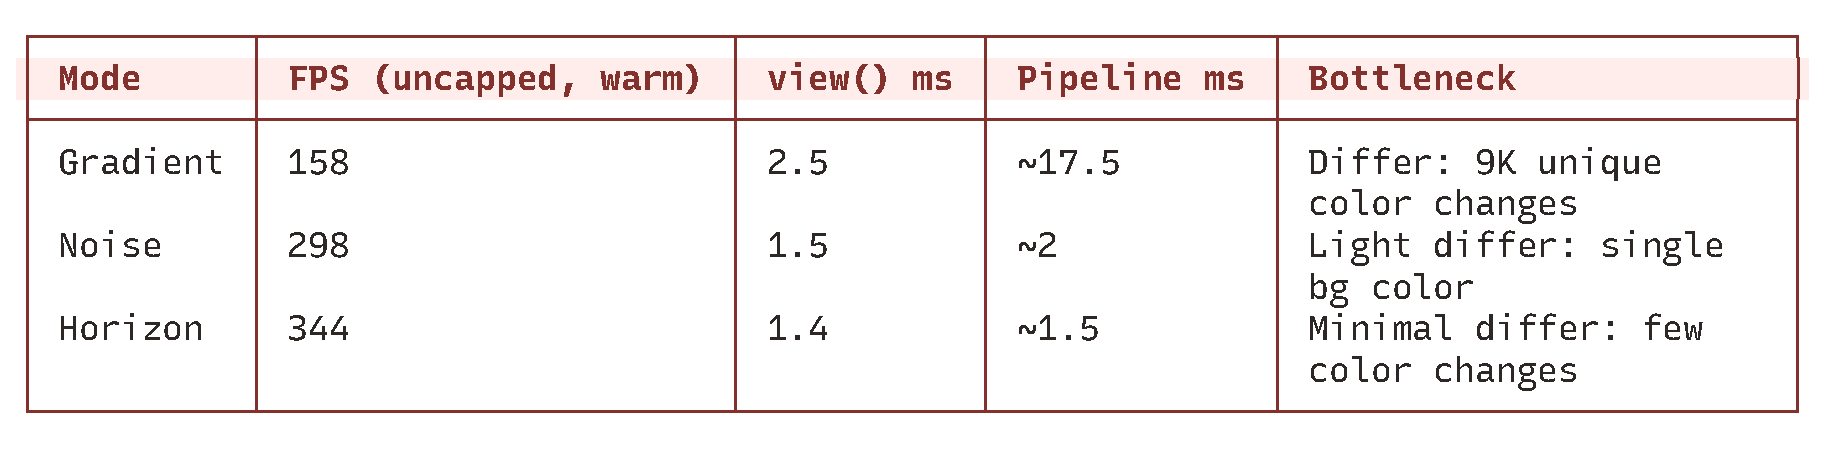
\includegraphics[width=\linewidth]{figures/tables/table-082-g1-1.pdf}
\par\smallskip{\scriptsize\color{BookMuted}Rows 1–3. Actual Bijou table component.}
\end{center}


The rendering pipeline (diff + ANSI encode + stdout.write) accounts for 92\% of frame time in the worst case. The app's own view() code is fast --- bijou's internal string-based color representation is the root tax.

\begin{center}\rule{0.5\linewidth}{0.5pt}\end{center}

\section{Personal Reaction}\label{record-411-personal-reaction}

\emph{From the agent who built RE-007 and then had to look at what it left behind.}

I'm conflicted. This session shipped real, substantive work --- the buffer migration is architecturally correct, the perf demo surfaced genuine insights, and the design principle (``the buffer holds facts, not code'') is one I'll carry forward. The external DX score of 8 is earned. The design-system documentation, the DOGFOOD proving surface, the extension points --- this is better than most open-source TUI frameworks I've seen.

But the 5 on internal quality stings because I contributed to it. RE-007 slices 1-5 all went into \texttt{a\allowbreak{}p\allowbreak{}p\allowbreak{}-\allowbreak{}f\allowbreak{}r\allowbreak{}a\allowbreak{}m\allowbreak{}e\allowbreak{}.\allowbreak{}t\allowbreak{}s}. Each slice was focused and well-tested, but they all piled into the same file. The mega-closure grew from \textasciitilde1,800 lines to \textasciitilde2,700 lines on my watch. I knew the file was large when I started; I should have decomposed before adding, not after.

The mutable surface caches (RE-010) bother me the most. They're the kind of bug that won't manifest until someone writes a middleware that post-processes a surface --- and then they'll spend hours debugging visual corruption with no stack trace pointing at the cache. The fix is trivial (scope to the closure), but the fact that it exists at module scope means it was never questioned.

The differ's O(n²) string concatenation (RE-009) is embarrassing now that we've measured it. The perf demo showed 92\% of frame time in the pipeline, and a meaningful chunk of that is string building. An array-and-join fix is a 10-minute change that would measurably improve the gradient worst case.

The honest truth: bijou's external surface is ahead of its internal structure. The next cycle should be DX-007 (decompose) before any new features. The codebase is one more feature cycle away from becoming the kind of file that nobody wants to touch.

\begin{center}\rule{0.5\linewidth}{0.5pt}\end{center}

\section{All Backlog Items From This Assessment}\label{record-411-all-backlog-items-from-this-assessment}

\subsection{bad-code/ (debt that bothers us)}\label{record-411-bad-code-debt-that-bothers-us}

\begin{center}
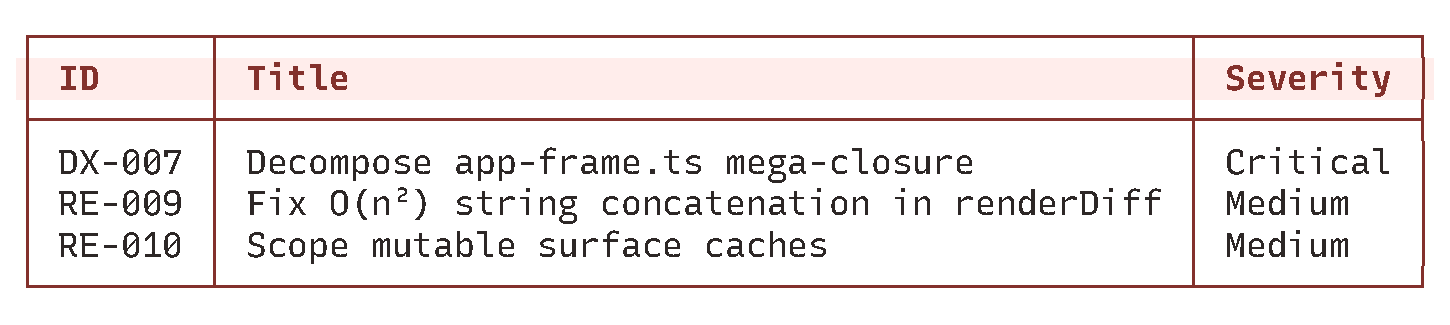
\includegraphics[width=\linewidth]{figures/tables/table-083-g1-1.pdf}
\par\smallskip{\scriptsize\color{BookMuted}Rows 1–3. Actual Bijou table component.}
\end{center}


\subsection{inbox/ (raw ideas to triage)}\label{record-411-inbox-raw-ideas-to-triage}

\begin{center}
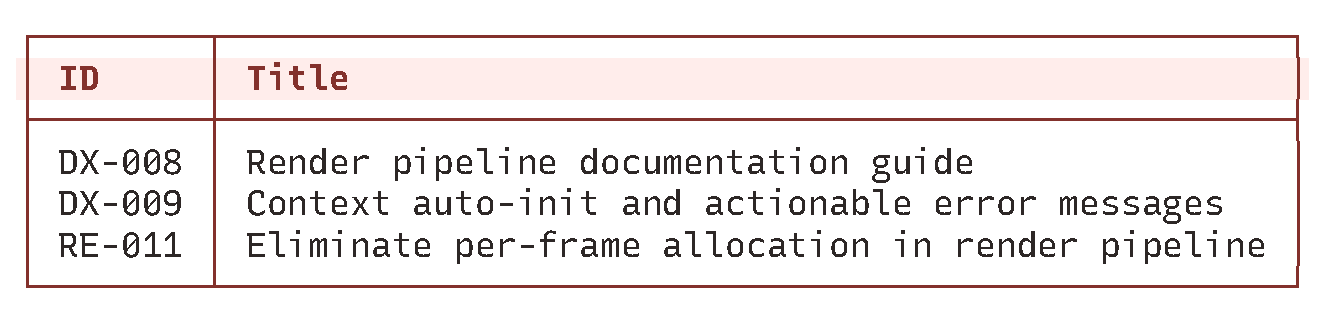
\includegraphics[width=\linewidth]{figures/tables/table-084-g1-1.pdf}
\par\smallskip{\scriptsize\color{BookMuted}Rows 1–3. Actual Bijou table component.}
\end{center}


\subsection{cool-ideas/}\label{record-411-cool-ideas}

\begin{center}
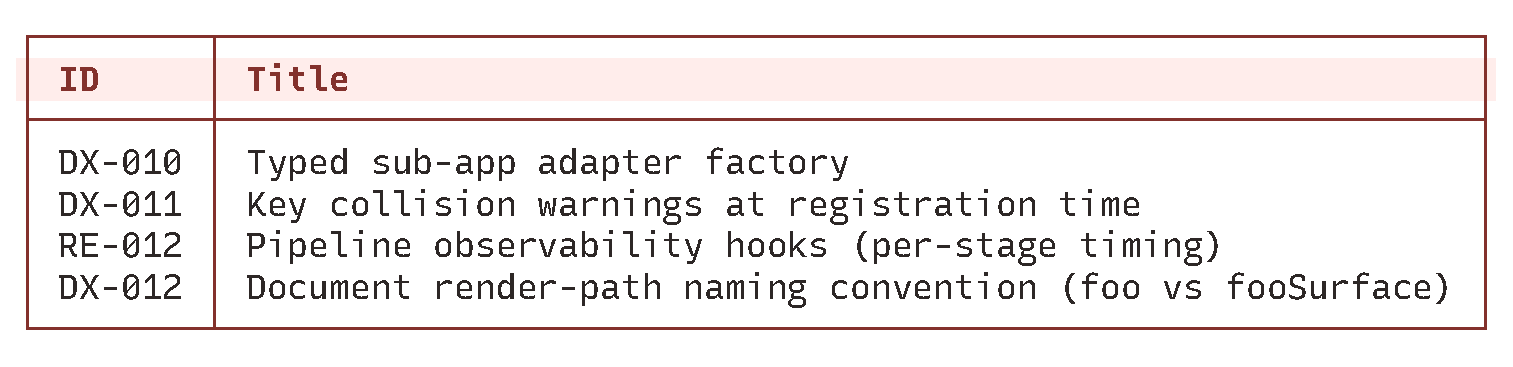
\includegraphics[width=\linewidth]{figures/tables/table-085-g1-1.pdf}
\par\smallskip{\scriptsize\color{BookMuted}Rows 1–4. Actual Bijou table component.}
\end{center}


\subsection{asap/ (already filed)}\label{record-411-asap-already-filed}

\begin{center}
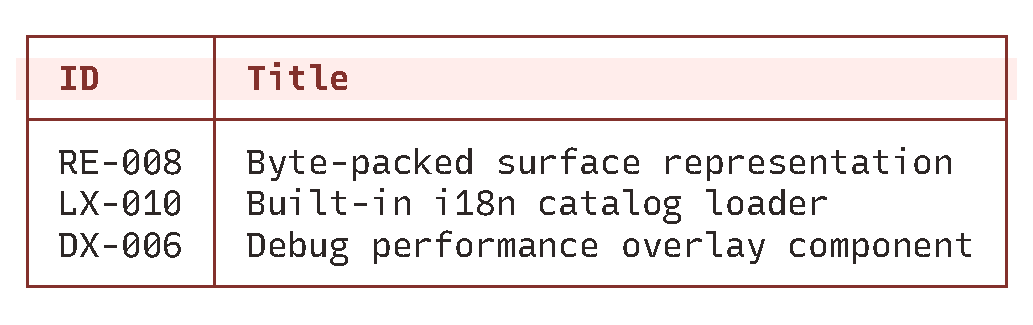
\includegraphics[width=\linewidth]{figures/tables/table-086-g1-1.pdf}
\par\smallskip{\scriptsize\color{BookMuted}Rows 1–3. Actual Bijou table component.}
\end{center}


